\documentclass[14pt]{extarticle}
\usepackage[utf8]{inputenc}
\usepackage{ngerman}
\usepackage{array}
\usepackage{amsmath}
\usepackage{graphicx}
\title{Bericht Todesstern U5 - Transformationen}
\author{Charline Waldrich, Robert Ullmann, Julian Dobrot}
\date{15. Dezember 2015}

\begin{document}

\maketitle
\pagebreak
\tableofcontents


\section{Aufgabenstellung}
Implementierung einer 4x4 Matrix, einer Klasse für Transformationen und einen Szenengraph. Desweiteren soll ein UML Diagramm gezeichnet werden, was den Raytracer nach den Änderungen durch diese Aufgabe wiederspiegelt.
\subsection{UML Diagramm}
Das Klassendiagramm abgeleitet aud der Aufgabenstellung von Übung 5.\\
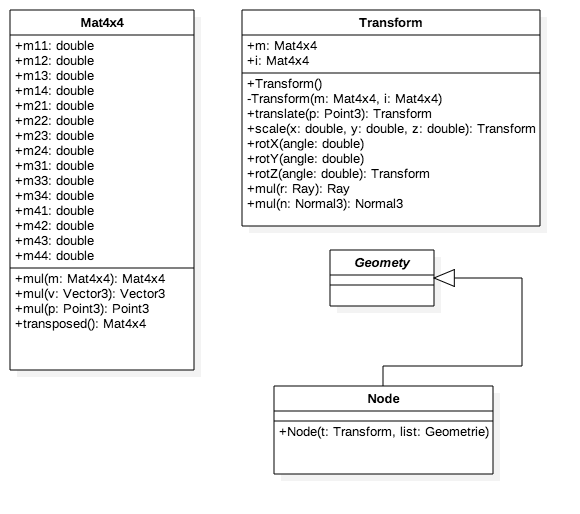
\includegraphics[width=15cm,height=15cm]{images/ClassDiagram}\\


\subsubsection{Anpassungen andere Geometrien}
Nach der Implemntierung des Szenengraphs und dessen Tests können die nun unnötigen Parameter bei den bestehenden Geometrien entfernt werden und können zu folgenden Werten geändert werden:

\begin{itemize} 
\item Beider Kugel für $\vec{c} :=\begin{pmatrix} 0 \\ 0\\ 0 \\\end{pmatrix} $  und für r = 1.
\item Beider Ebene für $\vec{a} :=\begin{pmatrix} 0 \\ 0\\ 0 \\\end{pmatrix} $ und für 
$\vec{n} :=\begin{pmatrix} 0 \\ 1\\ 0 \\\end{pmatrix} $
\item Beider Box für $\vec{a} :=\begin{pmatrix} -0,5\\ -0,5\\ -0,5 \\\end{pmatrix} $ und für
$\vec{b} :=\begin{pmatrix} 0,5 \\ 0,5\\ 0,5 \\\end{pmatrix} $
\end{itemize}


\subsubsection{Probleme und besondere Ereignisse}
 

\subsection{Lösungsstrategien}



\section{Zeitbedarf}
\begin{center}
\begin{tabular}{cr}
Änderungen an bestehenden Klassen \	&60 min	\\
Licht	  \	&240 min	\\
Material 	\	&180 min	\\
Welt \	&60 min	\\
Demo \	&240 min	\\
Bericht  \		&180 min	 \\
	\hline
	&960 min
\end{tabular}
\end{center}

\section{Quellen}

\end{document}
